\chapter{Research Avenues}
\label{ch:researchavenues}
% ##################################################################################################################

\hfill \textbf{Authors:} Kai Nagel, Kay W.\ Axhausen, Benjamin Kickhöfer, Andreas Horni

\begin{center} 
\includegraphics[width=0.3\textwidth, angle=0]{frontmatter/figures/MATSimBook} \end{center}

% ##################################################################################################################
The on-going work and the interest documented in the many scenarios shows 
that the system has not exhausted its possibilities as a platform for research on it and with it. 
This chapter wants to highlight some of them for further discussion and maybe action. 

% ##################################################################################################################
\section{MATSim and Agents}

% Q-learning: learn utility for each state-action pair
%
% utility learning: learn utility for each state
%
% difference: In the second case, need to have a model about the world.  I.e. need to know which actions lead to which probabilities for the next state.

% 20.2 passive learning in a known environment

% naive: proceed until terminal state, backpropagate utility to all previous states, average over all such utility values ever collected per state

% adaptive dynamic programming: U(i) = R(i) + \sum_j M_{ij} U(j)

% where R(i) is the reward at i and M_{ij} are the transition probas 
% (recall that this is passive learning)

% I don't that that this can be sampled ... needs to solve the equations

% temporal difference (TD) learning: U(i) <-- U(i) + alpha * ( R(i) + U(j) - U(i) ) 

% 20.3 passive learning in an unknown environment

% Since TD never neede M_{ij}, it will still work as before.  Will now also 
% learn M_{ij}, but separately

% 20.4 active learning in an unknown environment

% Now M^a_{ij} (depending on the action)

% U(i) = R(i) + max_a \sum_j M^a_{ij} U(j)

% TD approach same as before

% 20.5 Exploration

% 20.6 Learning an action-value function (Q values, Q-learning)

The core \gls{matsim} architecture---where agents learn utilities for plans---was originally derived from the so-called field of \acrfull{cas} \citep[e.g.][]{AxelrodBook,Holland_1992,HraberJonesForrestEcho,PalmerEtAl_PhysicaD_1994}. 
%% %\kwaah{Has this been spelled out somewhere ?} \ah{yes, gls()}
%% \kwaah{Why not Axelrod (1980) or Schelling: ``Schelling, TC 1978. Micromotives and Macrobehavior. Toronto, Canada: George J. McLeod Ltd.'' mit seinem Segregationsmodell} 
%% \ah{m.E. ist dies sein Seggregationspaper: \citet[][]{Schelling_TJMS_1971} (Issue 2), \citet[][]{Sakoda_TJMS_1971} (Issue 1) war aber sowieso vorher  gemäss Prof. Hegselmann.}
%% \kai{Müsste ich nach dem Urlaub machen.  \url{http://en.wikipedia.org/wiki/File:Map-of-complexity-science.jpg} gäbe ansonsten eine (m.E.\ ganz gute) Idee, welche Autoren man zitieren will.}
%
\citet{ArthurBar} addresses a coordination problem, where agents receive a payoff only when less than 60 out of 100 go to an event.  He addresses this by first generating a large number of heuristic predictors for the next round's attendance, such as ``same as in last round'' or ``trend of last four rounds''.  He next gives each agent a randomly selected handful of these strategies, so that agents in general have different sets of predictors.  Then, many rounds of the game are played, where the score of each predictor is updated based on its prediction quality,  
%\kwaah{payoff?} 
%\kai{nein, eigentlich so, wie es da steht: der score ($=$ payoff) wird angepasst basierend auf der Qualität der Vorhersage.  Wenn es unverständlich ist, was können wir dann tun?}
and agents act based on their currently best predictor.  Simulations demonstrate that the approach leads to successful coordination, \ie around 60\,agents show up in every round.
%
That approach in turn builds on work by \cite{PalmerEtAl_PhysicaD_1994}, who simulate a stock market, \citet{Holland_1992}, whose classifier systems have more structure than in Arthur's model but have a similar model of performance learning, or \cite{AxelrodBook}, who investigates adaptive agent in the face of repeated non-cooperative games.  

\citet{ArthurBar} kept each agent's predictors fixed after initialization.  In contrast,
\citet{HraberJonesForrestEcho} simulate an artificial ecosystem, where the individual agent strategies are based on so-called genes, which are adapted over the rounds/iterations by a genetic algorithms \citep{Goldberg_1989}.

The focus of \gls{cas} is on many agents, agent interaction, and emergence. \Gls{ai} in contrast concentrates on single agents. In \gls{ai} terms, the original \gls{matsim} agents (those that do day-to-day learning) are very simple 
%active 
reinforcement learning agents \citep[][Chapter 21.3]{RusselNorvig2010ArtificialIntelligence}. Since these \gls{matsim} agents have only one state (the initial/nightly state) and each action is simply a plan, the distinction between Q-learning and utility learning (as defined by \cite{RusselNorvig2010ArtificialIntelligence}) actually collapses, and what remains is the temporal difference 
%\kwaah{lagged} 
%\kwaah{Maybe better, given the difficult interpretation of the the iterations.} 
%\kai{Würde lieber bei ``temporal difference learning'' bleiben, denn das ist der terminus technicus.} 
learning (again as defined by \cite{RusselNorvig2010ArtificialIntelligence}) scheme for the utility, which translates to the \gls{matsim} situation which updates the score/performance/utility value of each plan every time it is selected.

\st{That is, overall,} \kai{von wem kommt das st?  warum?  Ich meine schon ``That is'', aber vielleicht ist der Text nicht klar genug?} the original \gls{matsim} system has inherited the focus on large systems, interaction, and emergence as well as the approach to strategy innovation from \gls{cas}, while the score updating rather comes from the field of \gls{ai}.

In consequence, a somewhat obvious path to move on is to include more aspects of modern \gls{ai} into the \gls{matsim} agents.  Examples include:
\begin{itemize}

\item Extend \gls{matsim} to agents that can react 
immediately, rather than having to wait for the next iteration or round.  In transport, this is sometimes called en-route or within-day replanning \citep[e.g.,][]{EmmerinkEtAl_TransResC_1995,balijepalli-2007}.  See Chapters~\ref{ch:withinday} and~\ref{ch:dts} as well as Section~\ref{sec:researchavenues-withinday}.

\item Improve the \gls{matsim} agents with respect to choice set generation.  This may include both a better creative capability of the agents to come up with innovative new strategies to handle their virtual lifes as well as considerations of consistency between choice set generation and estimated choice models.  See Sections~\ref{sec:Evolution-of-choice} and~\ref{sec:choicesets}.

\end{itemize}


%% In the meantime, both \gls{ai} and the field of transport simulation \st{have moved on}, \kwaah{switched their focus of interest} \kai{Ist das zwingend?  Ich finde ``have moved on'' eigentlich besser, weil es ja kein ``switch'' ist, sondern eine Fortsetzung. Vielleicht weiß jemand eine Formulierung, die weniger colloquial ist.} increasingly looking at agents that can react \kai{also below, chk}


%% \kai{to do more}

% ##################################################################################################################
\section{Within-Day Replanning and the User Equilibrium}
\label{sec:researchavenues-withinday}
Within-day replanning, \ie the ability of the agents to respond to the immediate context is the standard mode of operation for simulation models. 
%
In the transport domain, note the traffic flow models as an example, where aspects such as acceleration/braking or lane changing are (obviously) computed reactively while the simulation is running, and not before the simulation starts \citep[e.g.][]{Wiedemann_PhDThesis_1974}.
%
Many traveller-oriented or agent-based models of travel demand adopt the same approach (ORIENT \citep[][]{Sparmann_TechRep_1980}, ORIENT/RV \citep{AxhausenHerz_JTE_1989}, MobiTOPP \citep[][]{SchnittgerZumkeller_ETC_2004}).
%
For many aspects of \acrfull{its} systems, within-day replanning is indispensable \citep[e.g.][]{hall-1993,EmmerinkEtAl_TransResC_1995,Dobler_PhDThesis_2013}.
%
%% and all the work on intelligent transport system 
%% \kwaah{do we have more?})
None of these systems aim for equilibrium in the sense adopted by \gls{matsim} carried forward from \gls{transims} and ultimately inherited from static assignment.

One may argue that, if supplied with a learning approach, these within-day models should approach equilibrium after many iterations, as the agents with a suitable memory structure would avoid plans which make them worse off. 
%
This memory, which would need to be agent-specific and covering the very large set of choice options, makes the approach costly to implement.
%
Importantly, the solutions may be different: When faced with a stochastic environment, an agent that is able to react within-day can be better off than an agent that follows a pre-computed plan. \kai{!!!}

Still, there are context where this immediate response ability can be used within \gls{matsim} to explore the choice set more effectively, especially if the choice alternatives are limited in number and in geographic reach. 
\citet[][]{WaraichEtAl_TechRep_IVT_2013_2}
%Waraich et al. (200x) 
%\kwaah{What is the best reference here?} 
%\ah{afaik, this approach never come beyond a conceptual paper.}
proposes a 
%localized within-day, actually 
within-trip replanning to find the best parking space around a destination.
This localized search reduces the need for full iterations considerably and allows to add behavioral detail at this point, here the type of parking, walking distance to final destination, and parking fee trade-off. 
%In the same spirit, Horni (2015) \kwaah{Gibt es da schon etwas?} \ah{not yet} employs the same approach to address crossing of signalized intersections. 

While within-day replanning can be used as described above within the framework equilibrium search, it can also be added to open up the \gls{matsim} framework to context where such an equilibrium is inappropriate. 
%
\citet[][]{Dobler_PhDThesis_2013} uses the \gls{matsim} calculated equilibrium as the starting point for his model of evacuations and the behavior of the evacuees. 
He also documents that his approach finds a set of executed plans which is close to the \gls{matsim} equilibrium, but for much lower computing costs. 
While the benefits of an equilibrium solution in comparison with an approximation have been extensively discussed for aggregate assignment models, for \gls{matsim} the issue is if these fast approximation could be used to speed up the overall equilibrium search; similar in spirit to start a Frank-Wolfe search based on four or five incremental network loadings of the network.\kai{citation?}
While aggregate assignment has possibilities to identify the routes chosen as belonging to the equilibrium, in the agent-based context research is needed to a) see, if the approach is indeed faster and b) if the resulting set of plans is unbiased by the fast initialization. 

%\vfill\eject
% ##################################################################################################################
\section{Choice Set Generation}
\label{sec:choicesets}

\kai{in particular plans removal!!}

As described at several places in this book (e.g.\ Sections
\ref{sec:plans-gener-remov}, 
\ref{sec:Evolution-of-choice},
\ref{sec:choice-set}), the \gls{matsim} iterative process in its standard version modifies each agent's choice set ($=$ each agent's set of plans) over the iterations.  
%
Clearly, an agent can only select a plan that is generated by this process.  Thus, the definition of the search space is important.

Econometric research \citep[e.g.][Chapter 8 and 9]{BenAkivaLerman_1985} points out that it is not sufficient if certain alternatives are eventually discovered by the search process; rather, it is important that they are generated with statistical weights that are consistent with the choice model.
%
This, however, is somewhat at odds with the \acrfull{cas} approach, where solutions are generated somewhat arbitrarily.  For example, \citet{ArthurBar} ``create[s] `an alphabet soup' of predictors'' that are ``randomly ladle[d] out''.  That is, research is needed to clarify under which conditions the statistical properties of the choice set need to be tightly consistent with the choice model, and when not.

Having said that, in the \gls{matsim} context it turns out to be important to not only look at plans generation/innovation (e.g.\ Sections~\ref{sec:timechoice}--\ref{sec:modechoice}), but also at plans removal.  The default \gls{matsim} approach is to remove the plan with the worst score.  This is, however, problematic both from a \gls{cas} and an econometric perspective.



\kai{From Benjamin's diss:}

During the plans innovation process of the simulation, the plan with the lowest utility is removed whenever the maximum number of plans are reached for an agent. In consequence, this decreases the probability that heterogeneous plans survive and increases the probability of very similar plans. This, again, increases the likelihood that the final choice set is correlated, \ie containing only plans that are very similar to the best plan \citep[see][for a review on correlation of 
 routes]{Prato2009ChoiceModellingSurvey}.%
 %
 \footnote{
 %
 A possible solution to this problem is most likely composed of two steps:
 %
 First, more heterogeneity needs to be introduced into the choice set generation, \eg by producing very different plans.
 %
 Second, the method for plans removal needs to be based on an \gls{mnl} model where the difference in utility enters, similar to the approach of selecting plans for execution. This could be done by an implementation of a method called \gls{pathsizelogitmodel} which uses similarity measures for plans \citep[see][for a possible solution in route choice]{FrejingerBierlaire2007PathSizeLogit, BenAkivaBierlaiere1999DiscreteChoice}.
 %
 }

% --------
\kwaah{
No extended research has been undertaken so far to see, if \gls{matsim} could adopt the strategy of \glspl{ga}, which regularly introduce new random starting solutions to avoid local minima. 
The challenge is that the generation of such random plans would result in most cases in nonsensical plans, which would need to be removed through computationally expensive iterations. 
See \citet[][]{Feil_PhDThesis_2010} for the difficulties in constructing optimal alternative plans in terms of number and sequence of activities. 
One possibility is to allocate a small set of randomly chosen alternative day plans at the beginning and to measure their similarity throughout the simulation and to reduce the chances of their removal depending on their lack of similarity with the other plans. 
Furthermore, there is no research which has studied a replanning technique involving the switching of the activity order of the day plan, which again would produce more dissimilar plans than currently possible. 
}
%----------

To give recommendations to other researchers: the bias in choice set generation of \gls{matsim} needs to be fixed in the near future in order to obtain valid choice sets.
%
This requires (i) the generation of more heterogeneous plans \citep[see, e.g.,][for such attempts in the \acrshort{pt} and in the car mode, respectively]{Moyo2013PhD, NagelKickhoeferJoubert2014HeterogeneousVoTsPROCEDIA}; and (ii) the implementation of a \gls{pathsizelogitmodel} in the plans removal process \citep[see, e.g.,][]{Grether2014PhD}.
%
Having obtained these valid choice sets \citep{NagelFloetteroed2009IatbrResourceInBook}, the calculation of user benefits based on the \gls{logsum} formulation is preferable.
%
\benjamin{Well, here it now depends on how we write the previous section...}
%
Using the logsum formulation with correlated choice sets requires a careful interpretation of the results 
\kwaah{As far I can see, nobody has worried about this in ABM construction, as they assume that the nesting takes care of this, which it doesn't (fully)}. 
However, when looking at differences between the two states before and after a policy, this issue is unlikely to change results structurally: if the correlation remains roughly the same between the two states, the error of utility differences is small. If the correlation structure of plans changes, the error will\textemdash among other model specifications\textemdash depend on the number of iterations.
%
\benjamin{If we iterate the base case to the same iteration number as the policy case, the former will be more correlated. This would result in a underestimation of the utility changes.}
%
\kwaah{
– kwa: assuming we start with the equilibrium of the base case. This would result in an underestimation of the utility changes 
– kwa: assuming that the correlation means similarity and that the policy case has a tighter distribution.] 
}
In that sense, one could include some approximation of the error into the analysis of results, possibly similar to Equation~(\ref{eq:ch:economicEval:logsumMaxError}). If the differences in utility levels between the two states are in the same magnitude as $\ln(P)$, it is possible that the signal of the policy effect is smaller than the noise of randomness.

% -----------------
\kwaah{
The question of the need for a meta-search for strategies, as sketched by \citet[][]{ArthurBar} remains an open question. 
In the \gls{matsim} context all decisions, which are based on explicit search for alternatives, can be studied to see, how far apart the choice set generation strategies of discrete choice modeling, which draw (stratified) (randomly) from the universal choice sets, are from explicit construction strategies. 
The question would be in the second step to see, what impact these would have on the results and the policy conclusions. 

A good example is parking search \citep[][]{Waraich_unpub_IATBR_2012}, for which multiple strategies have been documented and which explain the empirical observations \citep[][]{Shoup_2005}. 
In a discrete choice model context, the distribution of parking preferences can mimic the choice strategies, but the approach would be unable to capture the context specific choice of the strategy. 
In \gls{matsim} this set of strategies could become the object of a meta-search to see, which agents would retain which strategies and how these would be used by the agents. 
Empirical work could be conducted to see, if these sets and their distributions match the travelers' practices. 

In the same vain, one could look at the destination choice for leisure, where different strategies can be observed, although they have not been subject of empirical study yet. 
If longer term choices were to be added to the \gls{matsim} framework, residential and workplace choice could also be considered. 

The issue of the convergence of the \gls{matsim} plans towards a single optimal structure, can be seen as the absence of search strategies on the plan level. 
This overlaps strongly with the question of the choice of the number and sequence of activities, where these alternative plans are needed. 
}

\kai{Finde ich interessant.  Hätte es aber gerne unter einer separaten Überschrift, irgendetwas mit ``search''.  Der ``agent''-Text, der dann erstmal nicht fertig geworden ist, sollte eigentlich eher in die Richtung gehen, wie ``autonom'' unsere Agenten eigentlich sind, also haben die eine eigene innere Uhr, haben die eigene Perception, berechnen die ihre eigenen Routen oder übernehmen sie Vorschläge, etc.  Falls obiges kein separates Kapitel wird, dann wäre es m.E.\ nur ein Teil von dem, was ich meine.}

% -----------------

% ##################################################################################################################
\section{Transients Versus the Notion of \enquote{Learning}}
\label{sec:transients-vs-learning}
As in many other simulations of similar kind, the interpretation of the relaxation procedure (iterations) of \gls{matsim} is unclear. 
%
Sometimes the relaxation process is ascribed a behavioral interpretation, for example, day-to-day learning, where also the transition process and not only the final equilibrium has a meaning \citep[][p.128]{LiuEtAl_TransResA_2006}, \citep[][p.523]{NagelBarrett1997feedback}. 
%
An opposite perspective exists, where the relaxation procedure is just a numerical method to compute the equilibrium state or states without a behavioral basis of the transitions.

%\vfill\eject
% ##################################################################################################################
\section{Utility Function}
\label{sec:future-of-scoring-function}
The current logarithmic \gls{matsim} utility function is not suitable for modeling activity sequence choice \citet[][p.127f]{Feil_PhDThesis_2010} and \citet[][]{MATSim_Userguide_2015}. 
Because of its negative second derivative, \ie its concavity, the log form favors very short activities, which means that the schedule is ever filled-up with short activities, where the usually long home activities are replaced first.%
\footnote{
With a fixed number of activities the log form optimum lies as far to the right as the overall budget constraint allows. 
In line with consumer theory's utility maximization, all first derivatives are equal and the unique optimum is stable.

With flexible number of activities their durations wander towards zero duration as the marginal utility is largest at zero, where zero duration itself is a singularity. 
Additionally, only the activity type with the shortest typical duration will survive the optimization process.} 
%
Since this generates completely unrealistic behavior, one is on the search for alternative functional forms. 

\ah{curvature param?}

% =========================================================================================
\subsection{Alternative Functional Forms of the Utility Function}
\label{sec:alternative-functions}
A new S-shaped function, proposed by \citet[][]{Joh_PhDThesis_2004}, was tested by \citet[][p.129ff]{Feil_PhDThesis_2010}. 
Establishing a positive second derivative near point of origin, by using an S-shaped utility function, is a natural idea to work against this degenerated mechanism of adding more and more and ever shorter activities. 
Estimates of the new function based on the Swiss microcensus were provided. 
This estimation, however, was difficult due to its non-linearities and the difficulty in generating sufficiently large choice sets. 
In addition many daily activities and their durations are not chosen freely by the individual. 
Without information about such constraints and social interactions the imposition of a utility maximizing framework is problematic. 
We and the literature have accepted this approach so far, but when we are addressing activity generation it might need to be rethought. 
Looking at the nested-logit-based activity based model literature it is obvious, that the generation and sequencing facets are mostly driven by the socio-economics of the travelers and the role of the logsum term summarizing the transport aspects is minor suffered inherent stability issues. 
Further tests with larger choice sets did not result in satisfactory results and further work has been stopped. 
Still, as induced and suppressed demand are urgent policy issues this stream of work would need to be taken up again. 

There are also technical issues with Joh's S-shaped formulation. % as detailed below in Section~\ref{sec:stabilityissues}. 
Away from the upper part of the curve, where it starts to become similar to a logarithmic curve, it grows very rapidly. 
In estimation this implies dramatic changes over short parameter spans. 
This makes finding an optimum difficult numerically. 
Additionally, the problem of the complete diminishing of those activities with longer typical durations, such as home activities, remains the same, when the number and types of activities is flexible.

It might be worth to take another approach based on the observation \citep[][and others]{SchlichEtAl_TransportRev_2004} that activity, location and mode form packages, which are rarely changed. 
One could think of the optimization task as a knapsack problem, where the traveler creates a Gestalt of the interactions to satisfy his commitments and his desires. 
\gls{tasha} is a model, which takes a similar stance. 

% ---------------------------------------------------------------------------------------------------------
%\subsubsection{Stability Issues With the S-Shaped Function}
%\label{sec:stabilityissues}

% ----------------------
%\ah{Some pieces of notes: Cannot put it down:
%
%Furthermore, an optimum with activity durations in the convex region of their utility functions is unstable. 
%...
%
%Either, (a) a small increase of their durations generates larger overall utility, than the shortening of the remaining activities in the concave region. Then the increasing curvature lets this activity increase further, or (b) the shortening 
%
%Furthermore, there are points where common system stability criteria---small perturbations only have small effects---is broken.
%At such points of the optimization trajectory, for filling up the time budget, it is suddenly better to add a new activity to the convex region than to prolong an activity in the concave region. \ah{ist immer so bei act repl}
%Due to the the S-shaped function's symmetry \ah{explain...symmetry not correct}, these points seem to fall together with the inflection points of the the bell-shaped first derivative of the S-shaped function.
%
% The optimization problem however, does neither have a stable optimum. An S-shaped function's first derivative is bell-shaped, \ie not bijective,
%
%The optimum is only kept, in the rare case, where the budget constraint exactly matches with all activities being at their utility function's inflection point, where the marginal utility is maximal.
%In all other cases ...
 %
%The maximum marginal utility is at the inflection point.
%
% The log forms first derivative $1/x$ is bijective.
%
%Together with the flexible number of activities, this means that there are infinitely many optima, \ie
%the time budget $T$ can be assigned to a variable number of activities in infinitely many ways representing an optimal plateau.
%
%with $N$ activities of which $m$ activities lie below injection point with first derivative $\cdot{f_0}$ and $N-m$ activities lie above injection point with first derivative $\cdot{f_1}$, 
%the total time budget $T$,
%and the infinitely small time change $dt$ 
%\begin{equation}
%m \cdot \dot{f_0}(t_0) \cdot dt = (N-m) \cdot \dot{f_1}(t_1) \cdot (T-m\cdot dt)/(N-m)
%\end{equation}
%has infinitely many solutions as $N$, $t_0$, $t_1$ are flexible; $t_0$ and $t_1$ are dependent on each other though.
%This also includes the case that activities have zero durations.
%In any case, it is very difficult to estimate such a function.
%Its behavioral suitability is another unsolved issue.
%
%\ah{ungewöhnliche Notation mit $dt$, wie schreibt man das sonst?}
%
%-------------
%
%consumer theory, first derivative equal -> defined clear optimization problem. 
%
%In other words, first derivatives do not need to be equal, 
%
%various combinations of activities lying above utility function injection point while others are below it are possible.
%
%This means that as long as the number of activities is flexible (degree of freedom) there exist ...
%
%The system is only stable (and optimal) if all non-zero-duration activities are exactly at inflection point of the utility function as detailed by following differentiation: 
%\begin{enumerate}
%\item All activities are in concave region (thus having equal marginal utility). Adding another activity might add additional benefit. 
%\item All activities are in convex region (thus having equal marginal utility). Removing one activity might add additional benefit.
%\item Some activities are in convex and others are in concave region. Increasing the convex activities while reducing the concave activities, or the other way round, might generate additional benefit.
%\end{enumerate}
%
%If one activity duration was in the convex region, then the overall utility could be increased by either
%(i) increasing its duration and at the same time reducing the duration of one activity in the concave region, or
%(ii) decreasing its duration and at the same time increasing the duration of one or more activities in the concave region.
%
%In any case; alle Ableitungen gleich stimmt nicht mehr
%
%If all activity durations are in the concave region (negative second derivative), another activity is added.
%If all activity durations are in the convex region (positive second derivative), at least one activity is set to zero 
%
%
%It does, however not prevent activities being set to zero duration.
%
%intuitively assigns the function estimates too much power.
%
%Problematic with this approach is the fact, that the system is only one stable point, the inflection point. 
%
%For the log function and at the optimal point all marginal utilities are equal. 
%
%Metaphorically speaking, the agent performs a system optimum search in terms of assigning time budgets to activities, where here system optimum is congruent with user optimum.
%
%
%For the S-shaped function system optimum is not necessarily congruent with user optimum, meaning that not all activities have equal marginal utilities at the system optimum point.
%
%In case the overall budget is too small to have all activities located in the concave region, there will be 
%
%There is no stable point in the convex region however. A stable point has $n$ activities in the concave region and $m$ activities at zero. 
%
%The gradient is positive but diminishing (second derivative negative). The system optimum view is congruent with the user optimum view.
%
%In the convex region. system optimum. Not all activities equal. gradient positive and increasing (second derivative positive). Pushed to zero nevertheless, if remaining activities in convex region generate more utility! Large depends on estimation. Only works correct in concave region.
%
%This is not a Lennard-Jones force!
%}

% ---------------------------------------------------------------------------------------
%\kai{Hallo Kay,
%Ist Euch die S-shaped utl function so wichtig, dass Ihr sie im "Buch" stehen haben wollt?
%Meine Intuition ist nämlich folgende:
%Es herrscht Wettbewerb zwischen Aktivitäten.
%Optimal ist wenn alle ersten Ableitungen nach der Zeit identisch (wie bei normaler consumer theory Ableitungen nach dem Preis).
%Theoretisch kann damit ein Arbeitspunkt auch im konvexen Teil der utl fct liegen.  Das ist aber instabil (siehe PS), und wird sich daher immer entweder nach Null oder in den konkaven Bereich bewegen.
%Damit gibt es aber auch in der Realität nur wenig oder gar keine Dauern im konvexen Bereich.
%Damit ist der konvexe Bereich nicht schätzbar.
%Insofern waren die Probleme bei Feil hier m.E. nicht Pech, sondern systematisch.
%Von mir aus kann sich die Welt damit trotzdem beschäftigen.
%Aber soll es wirklich als "research avenue" in das MATSim-Buch?  Oder könnten wir uns auf eine allgemeinere Formulierung einigen (wo wir einfach sagen, dass die derzeitige matsim fct zu unflexibel ist)?
%Danke \& vG
%Kai
%%
%PS: "Instabil": Sobald der Arbeitspunkt hier etwas nach rechts geht, geht die Steigung nach oben, der marginale Zugewinn steigt also an.  
%- Falls dieser Gewinn an Steigung mehr ist als der Verlust an Steigung an allen anderen Aktivitäten, dann wird der Anteil der betrachteten Aktivität immer größer, bis der Arbeitspunkt im konkaven Bereich ist.
%- Falls nicht, so gilt das Argument andersherum, und die betrachtete Aktivität wird auf Dauer Null zusammenschnurren.
%}

%\kai{Wir können aber auch unter research avenues durchaus so etwas wie "alternative functional forms of the utl function" als Überschrift nehmen, und dann kurz erklären, dass Feil es mit der Joh-Fkt probiert hat, aber mit einem Teil der Parameter Schätzprobleme hatte.  M.E. sollte nur das mit dem S nicht in der Überschrift stehen.}

% =========================================================================================
\subsection{Estimating a Utility Function}
\label{sec:estimation}
The challenge is that transport research has amply documented, that the travelers value different elements of their experience at different rates on average and certainly with large variances between each other. 
Some of these differences might be due to the omission of the daily schedule context, as well as missing interactions with the trip purpose and the omitted or misspecified distribution of the payment responsibilities (the firm paying, the parents paying for young adults, girlfriends paying for their boyfriends etc.). 
Still, the following differences should be accounted for: 
%
\begin{itemize}\styleItemize
\item Modal preferences either via modal constants or mode-specific valuation of in-vehicle-travel times to capture the comfort and social prestige effects
\item Walking time 
\item Transfers as a measure of their inconvenience and risk of the lost connection
\item Crowding above the disutility of the in-vehicle time for its discomfort
\item Parking search above the disutility of in-vehicle time for its uncertainty
\item Type preferences for parking places for the different levels of personal risk and risk for the vehicle
\item Cost sensitivity by available personal income 
\item Operating points for the activities
\item Level and curvature of the activity utilities by purpose
\end{itemize}

The literature has shown finer interactions, as well as further elements, but this set cover the key parts of the generalized costs. 
%As shown earlier, the commonly applied \gls{matsim} utility function parameters are derived from \citet[][]{ArnottEtAl_TAER_1993, ChaumetEtAl_2006}. 
\citet[][]{Kickhoefer_MastersThesis_2009} provides estimates based on data from \citet[][]{VrticEtc2008ReisekostenSVIBericht}. 
\citet[][]{KickhoeferEtAl2012WelfareBusCorridorKuhmoNectar} translates estimates from \citet[][]{TirachiniEtAl2012CrowdingCongestion} into \gls{matsim} values. 
However, with the exception of a few studies \citep[][]{BalmerEtAl_ResRep_datapuls_2010, HuelsmannEtAl2012HotspotPricing, KickhoeferNagel2013EmissionInternalizationNETS, KaddouraEtAl2015PtMarginalSocialCostPricingJTEP}, these estimates have not been considered yet for many other projects, although they represent a valuable base for future comparisons. 
The complete set outlined above has not yet been estimated in one consistent estimation, and so remains an urgent item for \gls{matsim} research. 

Having such a base at hand is important as estimating and applying a \gls{matsim} utility function is non-trivial due to the following. 

%
Agents optimize \emph{complete day plans} \citep[see also][Section 6.3.1]{MATSim_Userguide_2015}. This means that the utility levels of the single choice dimensions need to be carefully balanced, when applying estimates. Usually it is impossible to apply readily-available functions estimated independently for a single choice dimension. A degenerated example might be the following. All destination alternatives evaluated with a not-well calibrated utility function generate very low utility; in that case the complete activity might be simply dropped. 
%
\benjamin{I dont fully understand the above...what is an inappropriate utility function?} \ah{adapted}
%
This correlation or dependency between choice dimensions is also the reason why a day plan equilibrium does not necessarily include a Nash equilibrium for every single choice dimensions. 
The inseparability of choice dimensions means that in \gls{matsim} we can only consistently handle choices if the parameters are estimated or postulated consistently. 
Estimates from independent studies reflect the scale parameter of the Gumbel distribution of the observed choices, which is arbitrarily set to zero for identification purposes, which means that the values cannot be compared 
%\kwaah{(See Bierlaire, ????)}
. The elasticities and trade-offs values can be compared, as they removed the scale parameter from their values. 
%
\benjamin{Why? The only difference if one has more choice dimensions in the model is that utility differences resulting from some policy will be smaller than with less choice dimensions---\ie influencing the elasticity.} \ah{adapted}

Incorporating a contribution, \eg for parking or destination choice, in combination with absolute utilities is even trickier as the Charypar-Nagel function is non-linear, which means that available parameters---very often linear utility functions---need to be incorporated by approximation procedures and distinction of cases as described in \citet[][p.75ff]{Horni_PhDThesis_2013}. 
Furthermore, \gls{matsim} utility function includes travel times, while their parameters which are readily available from studies, the quality and potential bias in the calculation of the travel times used for those estimate is rarely challenged. 
It would be unlikely that these estimates are perfect, given that disaggregate assignment models have until recently only been calibrated against counts and not against observed travel times. 
The omission of junction models cannot help either. 
In addition, the travel time estimates are influenced by the underlying mode choice model in that implementation which can bias the results further \citep[][]{Vrtic_PhDThesis_2003}. 
\gls{gps} or smartphone-based surveys, however, provide this information with higher precision and, thus, they are a promising mean for better model calibration and therefore better description of the non-chosen alternatives in the model .

Furthermore, travel time and activity duration parameter estimates including income need to carefully consider the parameters' relation to the \gls{vtts}. \citet[][p.276]{MeisterEtAl_SVT_2009} for example argue that the average Swiss hourly earnings are much higher than 6\,EUR per hour used in the \gls{matsim} function then. 
However, the \gls{matsim} is now measured in utils not monetary units. 
Still, the parameters in utils and monetary terms (such as tolls, parking costs, fares etc., or income-dependent attributes) are often interacted and thus their relation needs to be consistent if they come from different studies.
%
\benjamin{I dont see the problem here...parameters define the \gls{vtts}, and are dependent on the variance of the unobserved attributes, no? So measuring in utils or money does not make a difference.} \ah{adapted}

%A numerical problem, particularly relevant for activity choice, concerns the functional form of the utility function---As argued in Section~\ref{sec:alternative-functions}, a function offering an additional degree of freedom (the curvature at the typical duration) would be better.

Estimating a utility function for \gls{matsim} is associated with another problem. 
The function is applied iteratively for a travel demand, which is in the beginning of the relaxation process usually not very similar to the situation for which the function was estimated. 
In other words, the function is used for a whole range of operating points, whereas it has been estimated for only one possibly completely different working point. 
The \gls{matsim} function thus must be also correct in the elasticities, to be able to efficiently drive the relaxation process toward the final relaxation point, where the estimated function is valid by construction. 

% =========================================================================================
\subsection{Agent-Specific Preferences}
\label{sec:agent-specific-prefs}
\gls{matsim} scenarios so far consider a relatively small set of agent attributes, essentially due to missing suitable data to derive detailed attributes for large populations \citep[][]{MuellerFloetteroed_unpub_hEART_2014}. 
Some studies, however, used larger sets of attributes. 
\citet{GretherEtAl2010TrbIncomeInTRR, KickhoeferEtAl2011PolicyEvaluationIncome} estimated individual income-contingent utility functions. 
\citet[][]{HorniEtAl_TechRep_IVT_2012_a, HorniAxhausen_TechRep_IVT_2014} incorporated agent-specific travel preferences and individual income-dependent marginal utilities of money; the preference values however, were assigned randomly. 
As natural consideration of agent-specific preferences is one of the corner-stones of agent-based \glspl{microsimulation}, future work should exploit this avenue. 

%\benjamin{Das haben wir auch gemacht -- vielleicht sogar noch ein bisschen genauer (mit HH-Einkommen und Lorenzkurve). Siehe \cite{GretherEtAl2010TrbIncomeInTRR, KickhoeferEtAl2011PolicyEvaluationIncome}. Da das früher war, vielleicht hier reinnehmen?} \ah{done}

% =========================================================================================
\subsection{Frozen Randomness for Other Choice Dimensions Than Destination Choice}
\label{sec:future-frozen-randomness}
For destination choice an iteration-stable random error term has been successfully applied to incorporate the unobserved heterogeneity not included by the stochasticity of the co-evolutionary process. Other choice dimensions, already implemented but in particular, future implementations concerning activity choice might also add explicit agent-specific error terms.  

A general implementation would obviously be useful. 
This implementation could incorporate a mechanism to generate the error terms with the correct correlation structures. 

%\vfill\eject
% ##################################################################################################################
\section{Double-Queue Mobsim}
\label{sec:researchavenues-double-queue-mobsim}
The standard \gls{matsim} \gls{mobsim} \gls{qsim} implements a single-queue model as described in Chapter~\ref{ch:kinematicwaves}. The associated \gls{fd} (flow vs. density) is horizontal for medium densities, and falls to zero very steeply at very high densities. This is consistent with the fact that a vehicle leaving a link opens up its space already in the next time step; jam patterns thus have a backwards traveling speed of $L/s$ ($L$ is the length of respective link) rather than the conventional approx. 15\,kilometers per hour.

The \gls{jdeqsim} (Section~\ref{sec:using-jdeqsim}) and the deprecated \gls{deqsim} (Section~\ref{sec:deqsim}) implement a double-queue model with backward traveling gaps. Currently, implementation work and tests are performed to include this also in \gls{qsim}; performance problems with the inclusion of a large number of holes is the remaining issue to be solved.

%\kai{Siehe auch Material in basicprocedure.tex}
%
%Illustrates empirically the summary in Section~\ref{sec:kinematicwaves-summary}.
%\ah{
%\subsection{Aggregate Traffic Flow Characteristics}
%\gls{matsim}'s aggregate traffic flow characteristics were analyzed in the common form of the macroscopic fundamental diagram. Some investigations additionally derived \gls{matsim}'s (implicit) volume-delay function \citep[][]{HorniMontini_STRC_2013}.
%
%Some simulation investigations had problems to reproduce the complete MFD (project NetCap, personal communication, 2014), in particular, the high density region. They used mobsim versions without the backward moving gaps feature. Other studies, based on DEQSim and JDEQSim respectively, which both \emph{do} include \emph{back moving gaps}, were able to generate realistic MFDs. \kai{Das ist natürlich kein Wunder.}
%
%\citet[p.81ff][]{Simoni_MastersThesis_2013} investigates \gls{matsim}'s ability to model macroscopic characteristics with a four link ring scenario. He found considerable influence of the backward moving gaps speed on the form of the MFD. \citet[][]{CharyparEtAl_TRB_2009} also use a circular toy scenario. They also found the typical trapezoidal form for a broad range of network resolutions.
%
%Natural conclusion here is, that back moving gaps are essential for generating a realistic MFD \kai{bis hier hin stimme ich zu}, in other words to realistically model the complete range of traffic conditions \kai{hier eigentlich nicht wirklich.}. Backward moving gaps are re-included in the default \gls{matsim} mobsim (qsim).
%}
%
%\ah{following copied from atlassian:}
%
%\kai{The queue model fundamental diagram (flow vs density) is horizontal for medium densities, and falls to zero very steeply at very high densities.
%This is consistent with the fact that a vehicle leaving a link opens up its space already in the next time step; jam patterns thus have a backwards travelling speed of ``length\_of\_link''/1sec rather than the conventional approx. 15km/h.
%
%A fix, developed by Charypar, is to generate a ``hole'' when a vehicle leaves a link, and have it travel with a configured velocity against the direction of traffic. The hole cannot be used before it has arrived at the upstream end.
%
%Now the problem is that the model is initialized with one hole per empty space. This means many ``hole'' objects which consume a lot of memory ... in fact, too much of it.
%Way out: Just keep track of the number of available holes. Initially, that number corresponds to the storage capacity. Every time a vehicle enters, the number is decreased (which can also take care of different vehicles sizes, \ie decrease by the PCE instead of by one). Every time vehicle leaves, a hole is created (with size equal to the vehicle's PCE) which travels upstream. When the hole has reached the upstream end, the number of available holes is increased accordingly, and the hole object is destroyed.
%This would need to be implemented and tested ...}
%
%\marcel{
%Having the holes only while traveling back brings it closer to an events-based implementation: Basically, the hole then represents nothing else as a delayed event to increase the available space on the link. This leads to a further simplified implementation: Instead of hole objects, one could just have a queue where the time, when an additional space becomes available (=when the hole would reach the start of the link), is stored. In each step, the head of the queue could be checked to see if space becomes available and increase the counter. This would then also be more queue-like like the name of the QSim suggests}
%
%\kai{
%Generelles Problem ist, dass nur die jdeqsim die double-ended queue implementiert, die normale QSim tut das derzeit nicht.  Es gibt seit dem dev mtg eine experimentelle Version für die QSim, aber die verbraucht so viel Speicher, dass man sie nicht empfehlen kann.  Habe jetzt Amit hinzugezogen, damit er mir dabei hilft; keine Ahnung, ab wann wir das evtl. fertig haben könnten.
%}

% ##################################################################################################################
%\section{Synthetic Population Generation}
%Müller
%\ah{not at the core of MATSim, maybe in a next edition}

% ##################################################################################################################
\section{Considering Social Contacts}
Apparently, social contacts, within households and within extended social networks have a substantial influence on travel decisions, in particular for social activities in leisure time \citep[][]{KowaldEtAl_unpub_STRC_2009}.
An early social networks study in context but not based on \gls{matsim} is \citet[][]{MarchalNagel_TRR_2005}.
Further work based on or, again, in context of \gls{matsim} was undertaken by \citet[][]{Hackney_PhDThesis_2009, IllenbergerEtAl_TechRep_VSP_2010, KowaldEtAl_unpub_STRC_2009, KowaldEtAl_ASNA_2009}.
Most recent work on joint trips is reported in Chapter~\ref{ch:jointtrips}. 
Despite this range of valuable work, future work is required on this topic in particular for leisure destination choice \citep[][]{Horni_PhDThesis_2013}.

%\vfill\eject
% ##################################################################################################################
%\ah{Habe Results' Variability auskomentiert.
%Das Zeug ist nur als STRC-paper publiziert, ist also nichts was die Welt vermissen wird.
%Zudem, ist es mir einfach nicht wohl dabei. Ich habe nicht die geringsten Sicherheiten, dass da nicht noch ein versteckter Bug kräftig mitrauscht.
%Frühere Arbeiten \emph{ohne} Zielwahl kamen auf viel geringere Samplingfehler, also hat man auch durch Kontext keine Anhaltspunkte.
%Zu guter Letzt ist das Ganze jetzt ja zumindest theoretisch in MC abgehandelt.
%}

%\section{Results Variability}
%\label{sec:variability}
%\Gls{microsimulation} system design as well as concrete \gls{microsimulation} studies require specification of the quantities of interest.\footnote{%
%Formal system specification (and verification) is discussed, \eg in \citet[][]{FisherWooldridge_IJCIS_1997, BourahlaBenmohamed_ENTCS_2005}. 
%} For microsimulation design, they need to be general and broadly available, count data are an example. For specific experiments and purposes other measures might be added; \citet[][]{Kitamura_TMIP_1996}, for example, lists measures relevant for emissions modeling. Considering their scale is important for model development, but a certain lack of research exists in this regard. \citet[][Section 2.2]{NagelAxhausen200Xiatbr00-report}, for example, say: ``Another question regarding scales is which scale is necessary to answer which question. There is wide-spread intuition but currently little hard knowledge. Rules-of-thumb, such as to include one level of resolution below the level of interest, are just rule-of-thumb.'' 
%
%Scale of the measures of interest is also relevant for results production, as different scales or resolution levels usually lead to different levels of \emph{variability} and, thus, to different study costs in terms of required computation effort. Transport microsimulations are usually stochastic. Randomness is, for example, introduced by the error terms of discrete choice models, a common component in utility-based \glspl{microsimulation}. This leads to random variability in results. Parameters or population statistics, such as averages, thus, need to be estimated by random sampling. \Glspl{microsimulation} are thus essentially a sampling tool \citep[][]{WolfDA_CSP_2001}, where one run represents one sample unit (in statistical terms one \emph{realization of a random variable}). This makes clear, that the whole toolbox used for other statistical methods, must be applied also here. As a first step, required sample size---here, the number of runs---to ensure a given confidence in the calculated averages needs to be calculated. In this context, variability is often seen as something tedious, because higher variability leads to larger minimal sample sizes, with usually relatively high costs per sample point. But, this view falls short. Clearly, unobserved variability---modeled as random variability---should be replaced to the extent possible (by explaining it). However, when looking at the very large proportion of temporal variability actually present in reality (Figure \ref{fig:counts}), a substantial part of this variability is---even if it was actually explicable---much more efficiently handled by including randomness, as model complexity would be prohibitively large otherwise. In this sense, \glspl{microsimulation} are a tool to capture these real-world fluctuations \citep[][p.11]{NewmanMEJBarkema_1999}, \citep[][p.704]{EsserNagel2001iatbr00-book}. This means also that the focus should not only be on averages, but also on variance incorporated in the calculations of statistical confidence. The following sections broaden the microsimulation variability analysis.
%
%\createfigure[!t!]%
%{Measured volumes}%
%{Volumes. LEFT: Reality.  RIGHT: Simulation. \kai{Hallo Andreas, mitteln die Messungen aus der Realität über alle Tagestypen einschl.\ Samstag, Sonntag, Ostern, Weihnachten, etc.?} \kai{Falls ja, so würde ich sagen, dass das dann ohnehin schwer zu vergleichen ist, und auch erklärt, was man sieht: In den realen Daten vor allem die Schwankungen zwischen den Tagestypen, womit dann die "daily" Schwankungen nicht kleiner sind als die "hourly".  In der Simulation hingegen Monte Carlo noise, der erwarteterweise kleiner wird, wenn man über 24h mittelt.}
%\ah{Die Analyse ist ein Weilchen her. Sehe aber, dass ich die Zähldaten-Dateien für diese Boxplots mit dem gleichen Package (playground.anhorni.counts) erstellt habe, wie die Counts für MATSim. 
%
%Würde also etwas Geld darauf wetten, dass ich auch den gleichen Filter angewendet habe, wie für die Zähldaten (Sa, So, Mo, Fr, Feiertage, Ferien sind somit nicht drin). Argument war damals: Warum um Himmels Willen wollen wir den (Zähldaten-Durchschnitt so genau treffen, wenn wir über mit der Mikrozensus-Nachfrage ein ganzes Jahr reinmixen, was in Realität offensichtlich große Varianz verursacht?
%
%Falls wir es genauer wissen wollen, kann ich das überprüfen/reproduzieren; ist alles als Skript vorhanden.}
%}%
%{\label{fig:counts}}%
%{%
%% ===
	%\createsubfigure%
  %{Daily Volumes}%
%
%{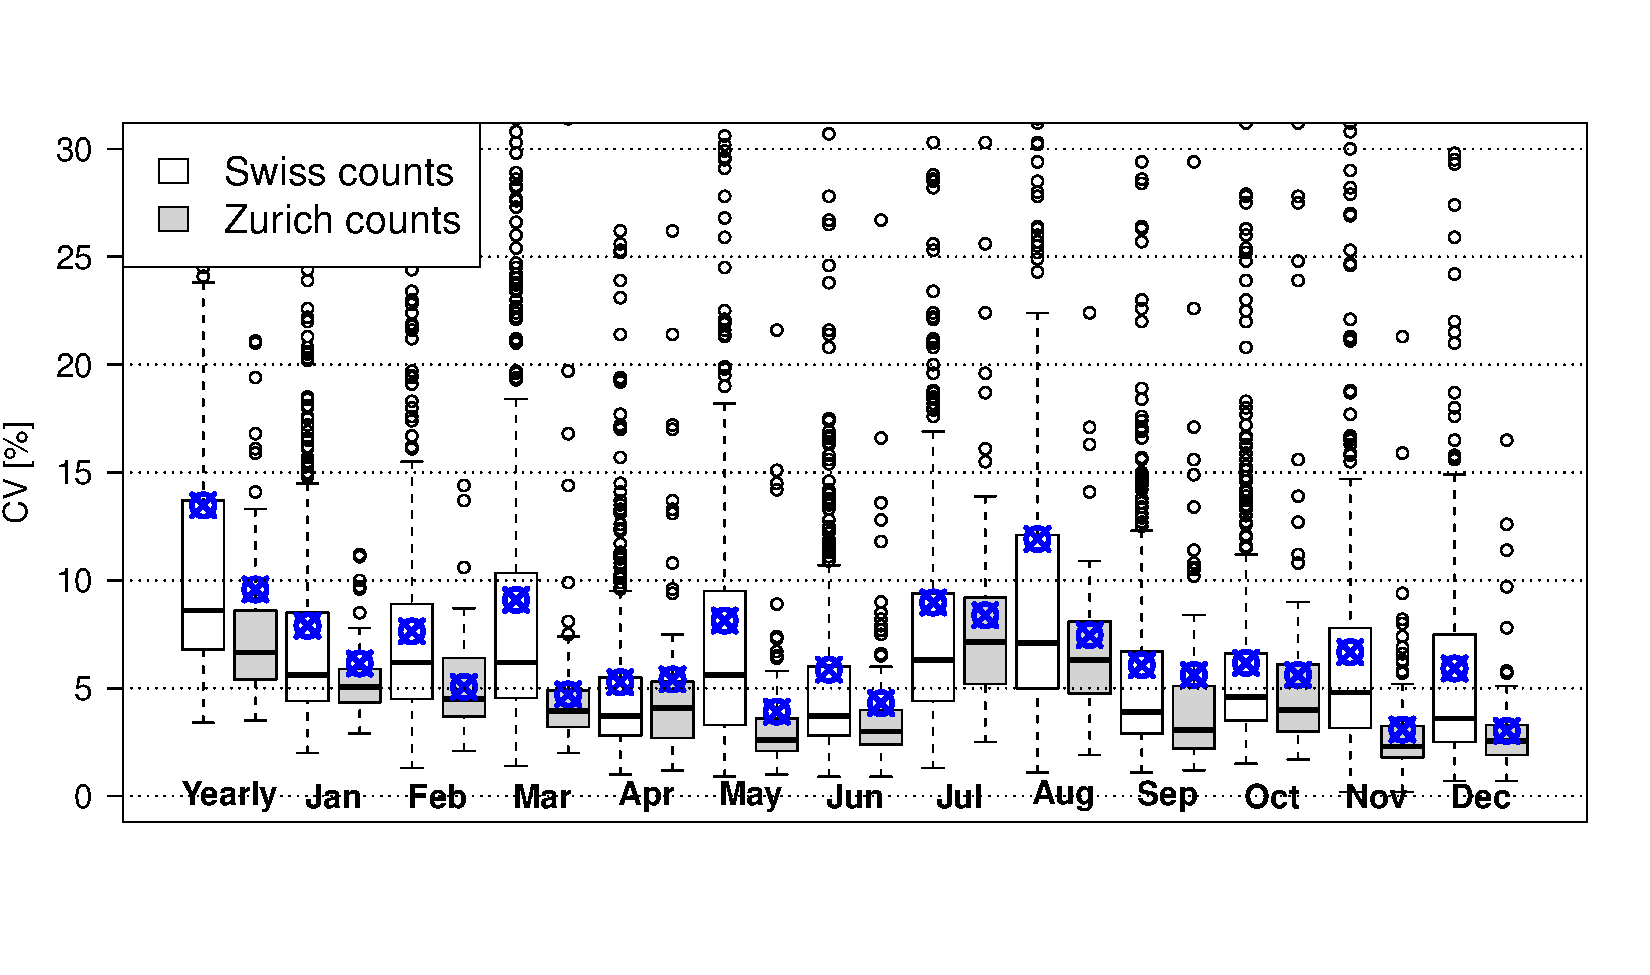
\includegraphics[height=0.3\textwidth]{understanding/figures/var/countsDaily.pdf}}%
	%{\label{fig:countsDaily}}%
  %{}%
%% ---
	%\createsubfigure%
  %{Simulated Daily Volumes: Inter-run Variability, runs~0-29, iteration~200}%
	%{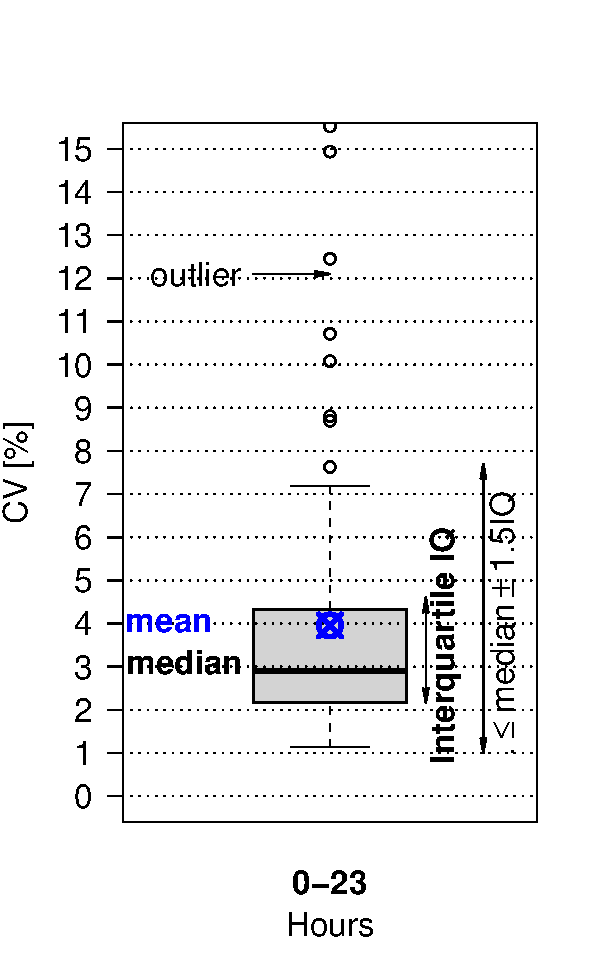
\includegraphics[height=0.3\textwidth]{understanding/figures/var/linkVolumesInterAWTV200.pdf}}%
	%{\label{fig:linkVolumesInterAWTV200}}%
  %{}%
%% ===
  %\createsubfigure%
  %{11:00-12:00}%
	%{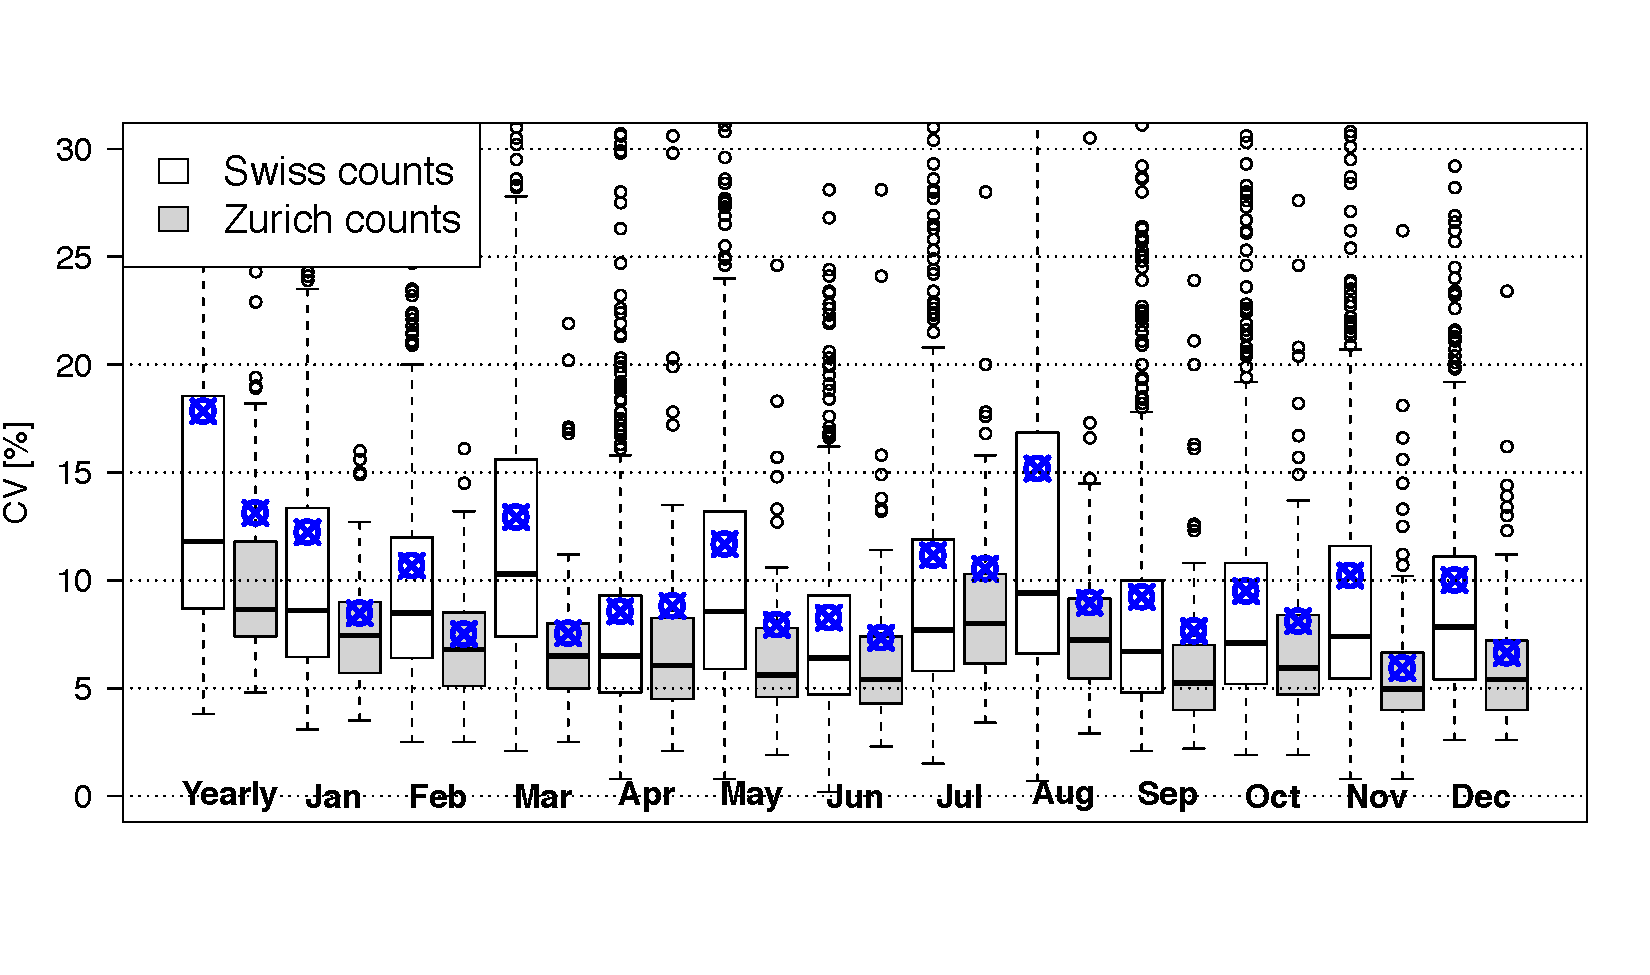
\includegraphics[height=0.3\textwidth]{understanding/figures/var/counts11-12.pdf}}%
	%{\label{fig:H1112}}%
  %{}%
%% ---
	%\createsubfigure%
  %{Simulated Hourly Volumes: Inter-run Variability, runs~0-29, iteration~200}%
	%{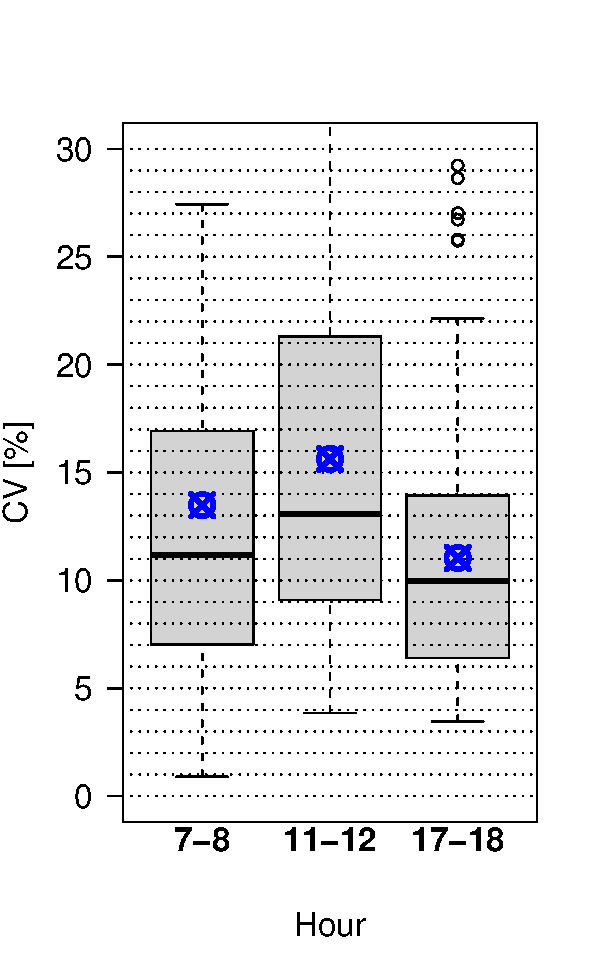
\includegraphics[height=0.3\textwidth]{understanding/figures/var/linkVolumesInter200.pdf}}%
	%{\label{fig:linkVolumesInter200}}%
  %{}%
%% ===
 	%\createsubfigure%
  %{17:00-18:00}%
	%{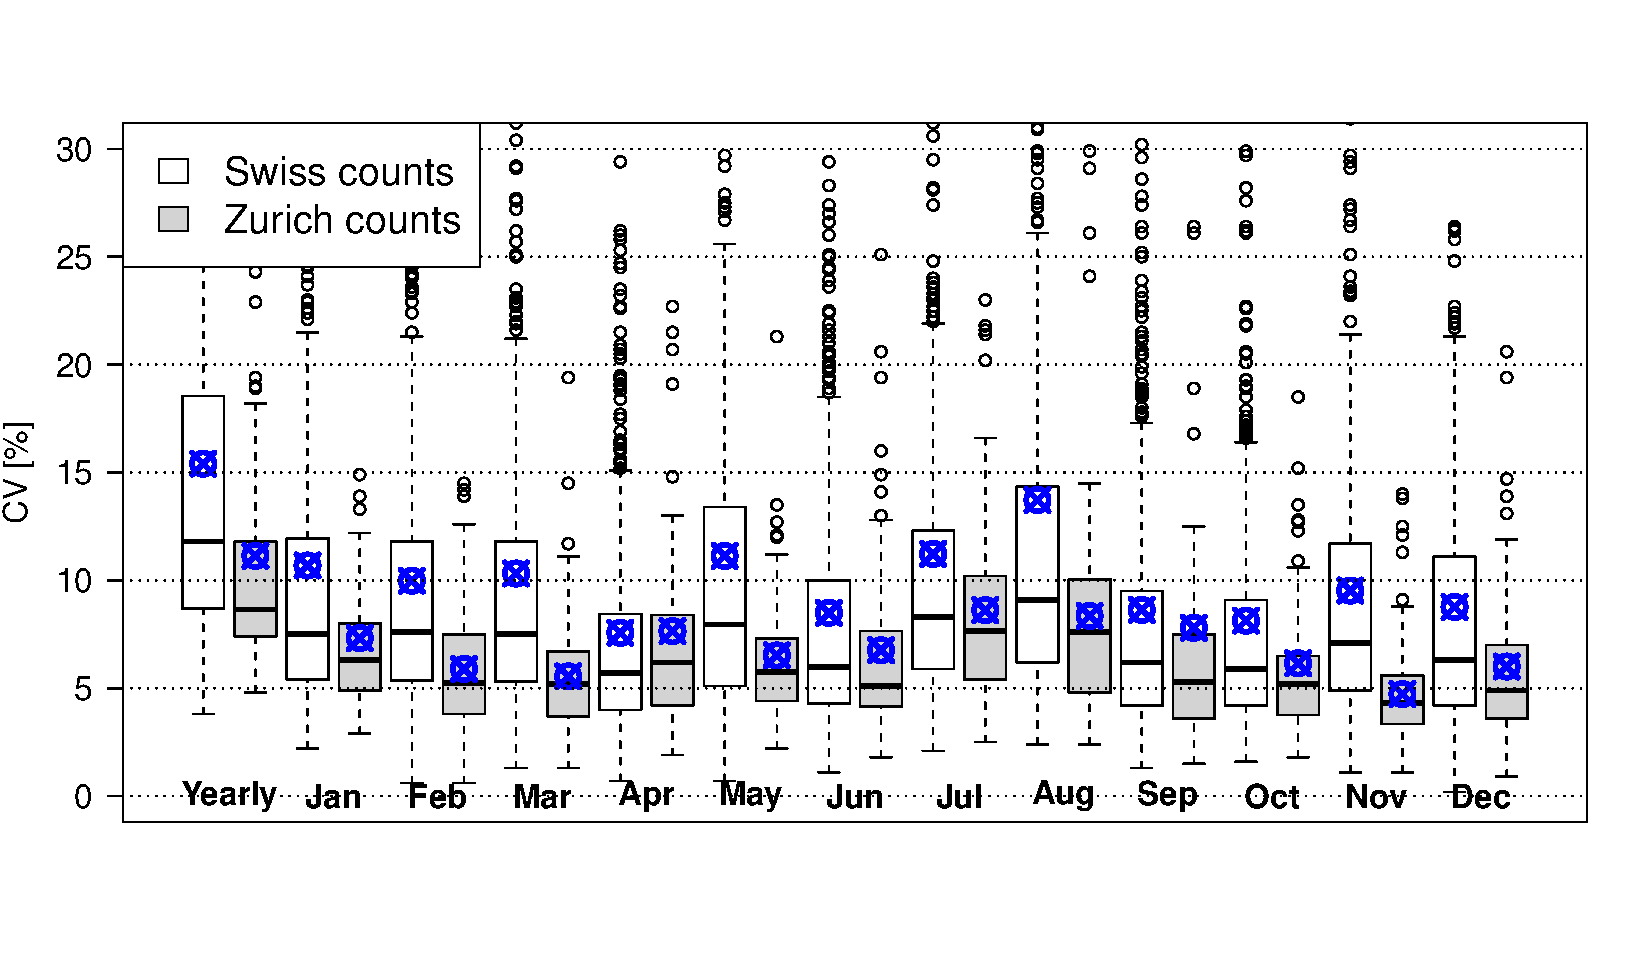
\includegraphics[height=0.3\textwidth]{understanding/figures/var/counts17-18.pdf}}%
	%{\label{fig:H1718}}%
  %{}%
%% ---
	%\createsubfigure%
  %{Simulated Hourly Volumes: Inter-run Variability, runs~0-29, iteration~200}%
	%{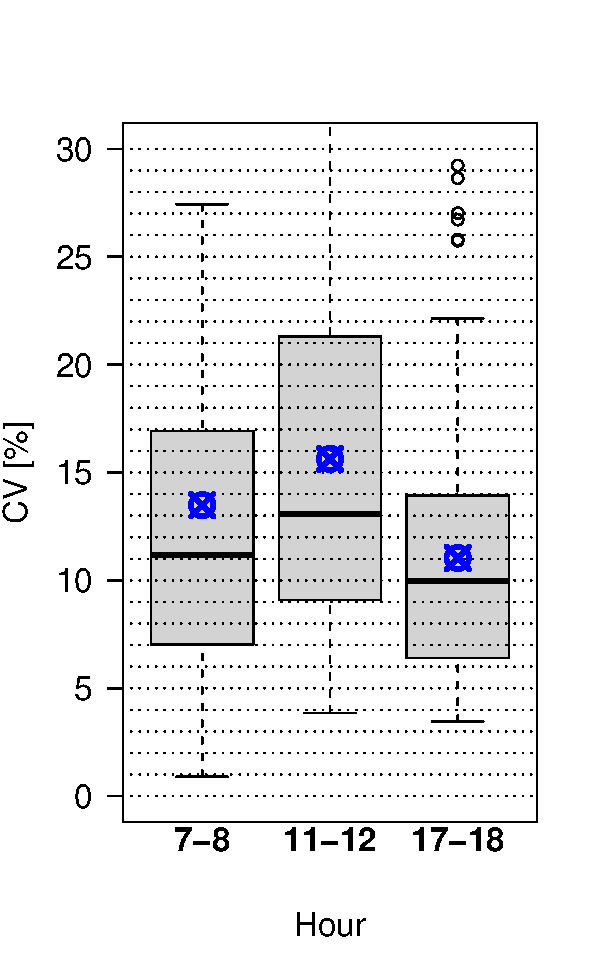
\includegraphics[height=0.3\textwidth]{understanding/figures/var/linkVolumesInter200.pdf}}%
	%{\label{fig:linkVolumesInter200}}%
  %{}%
%% ===
%}%
%{}
%
%Multiple possibilities to categorize microsimulations variability exist; some categories are described by \citet[][]{HorniEtAl_TechRep_IVT_2011_b}. Often a distinction between endogenous (model) variability and exogenous (input) variability is made. Equally suitable one can distinguish systematic and random variability. The experiments reported below mainly focus on \emph{random, endogenous} model variability. Random variability stems from inherently random choices and from actually systematic choices not recognized as systematic by the modeler.
%
%MATSim variability was investigated by \citet[][]{HorniEtAl_TechRep_IVT_2011_b, HorniEtAl_STRC_2011, Dayte_TechRep_IVT_2012} coming to the conclusion that at the population level, as expected, there is little variability between simulation results. Little variability exists likewise for \emph{daily} volumes as shown in Figures \ref{fig:linkVolumesAWTVInterScatter} and \ref{fig:linkVolumesInterAWTV200} (with a different visualization), which is consistent with previous work. However, the variability for \emph{hourly} volumes is an issue as shown in Figures~\ref{fig:linkVolumesHour17-18InterScatter} and Figure~\ref{fig:linkVolumesInter200} (with a different visualization).
%
%To interact these substantial simulation variability with variability observed in reality, \citet[][]{HorniEtAl_STRC_2011} looked at real-world link volumes given for both, the complete year and single months, meaning that a single point in the box plot represents temporal variability of a single network link, either for the whole year, or for a specific month. The hours 11-12 and 17-18 are shown as examples in Figure~\ref{fig:counts}, where similar patterns could be observed for all hours. The plots allow the conclusion that also in reality variability is also substantial.
%
%Further MATSim investigations are reported by \citet[][]{Hackney_PhDThesis_2009, Neumann_PhDThesis_2014}.
%
%\createfigure%
%{Simulated link volumes}%
%{Simulated link volumes}%
%{\label{fig:linkVolumes}}%
%{%
  %\createsubfigure%
  %{Simulated Daily Volumes: Inter-run Variability}%
	%{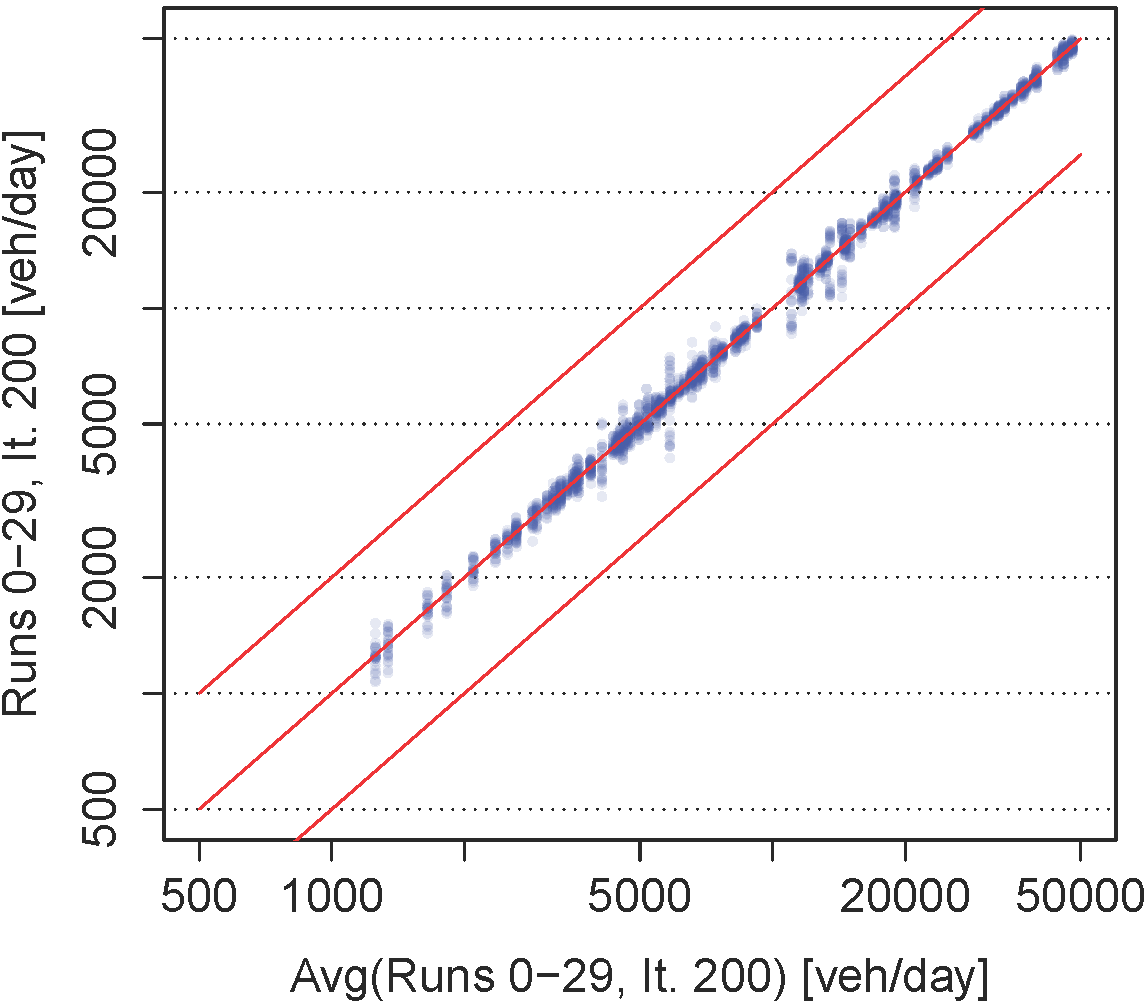
\includegraphics[width=0.49\textwidth]{understanding/figures/var/linkVolumesAWTVInterScatter.png}}%
	%{\label{fig:linkVolumesAWTVInterScatter}}%
  %{}%
	%\createsubfigure%
  %{Simulated Daily Volumes: Inter-run Variability, Runs 0-29, Iteration 200}%
	%{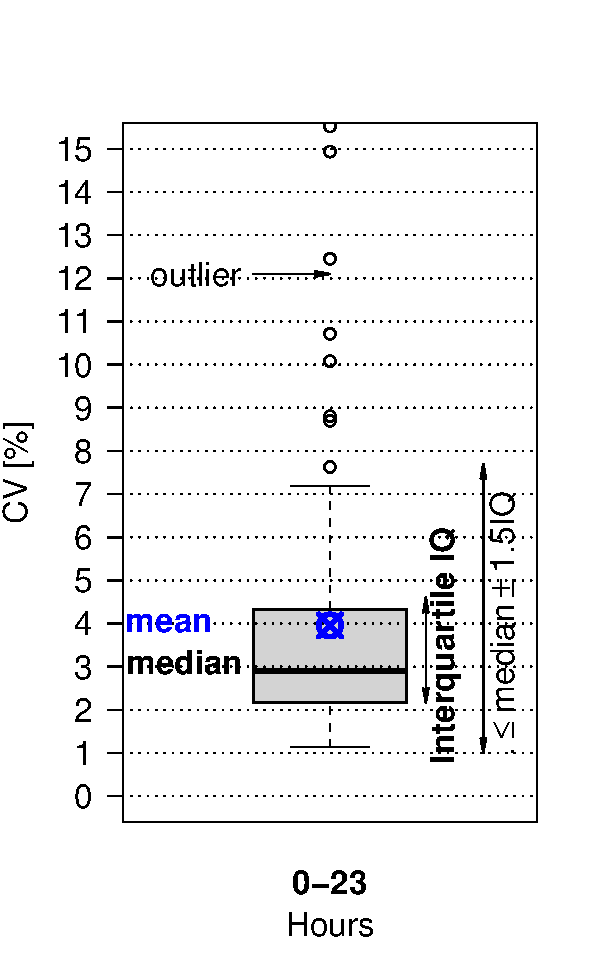
\includegraphics[width=0.3\textwidth]{understanding/figures/var/linkVolumesInterAWTV200.pdf}}%
	%{\label{fig:linkVolumesInterAWTV200}}%
  %{}%
  %\createsubfigure%
  %{Simulated Hourly Volumes (Hour 17-18), Inter-run Variability}%
	%{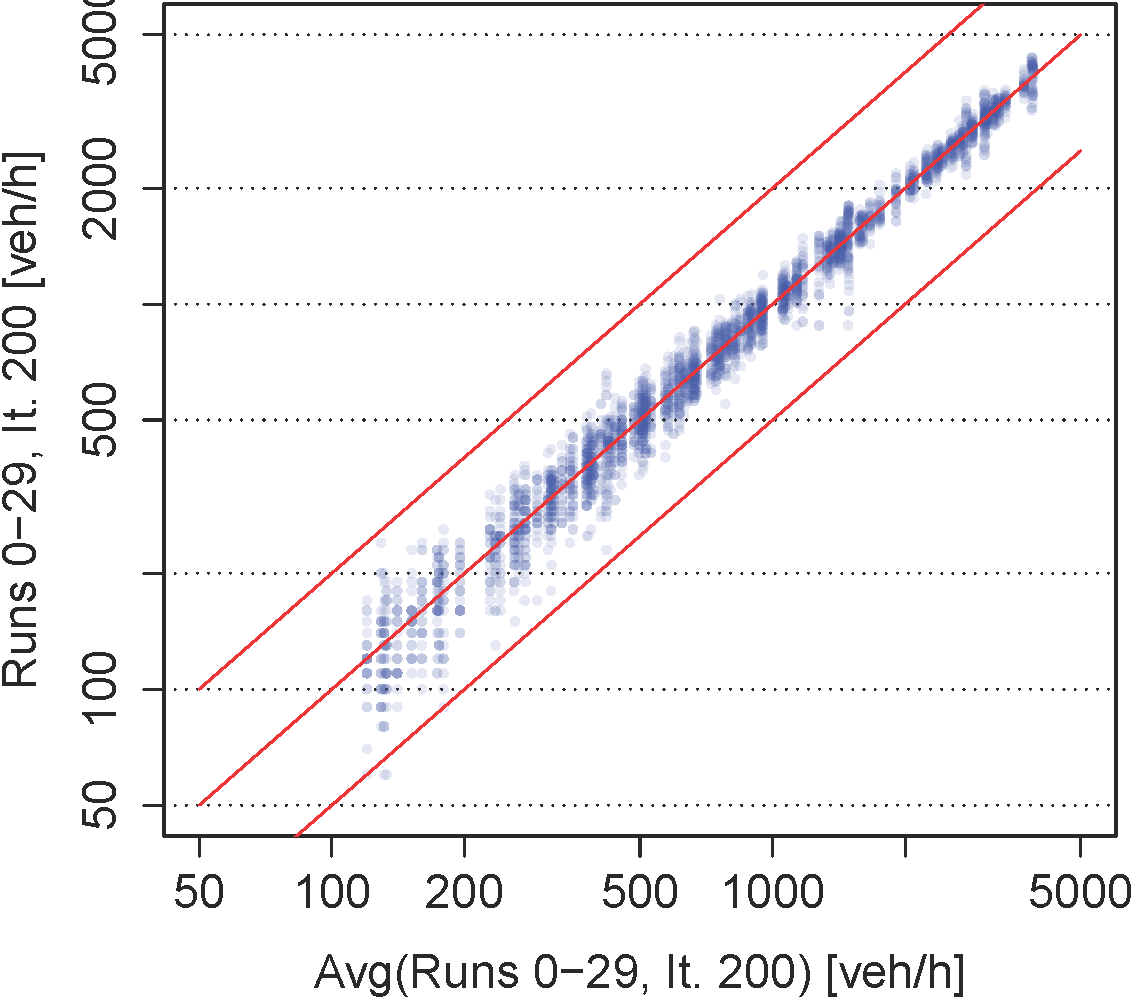
\includegraphics[width=0.49\textwidth]{understanding/figures/var/linkVolumesHour17-18InterScatter.png}}%
	%{\label{fig:linkVolumesHour17-18InterScatter}}%
  %{}%
	%\createsubfigure%
  %{Simulated Hourly Volumes: Inter-run Variability, Runs 0-29, Iteration 200}%
	%{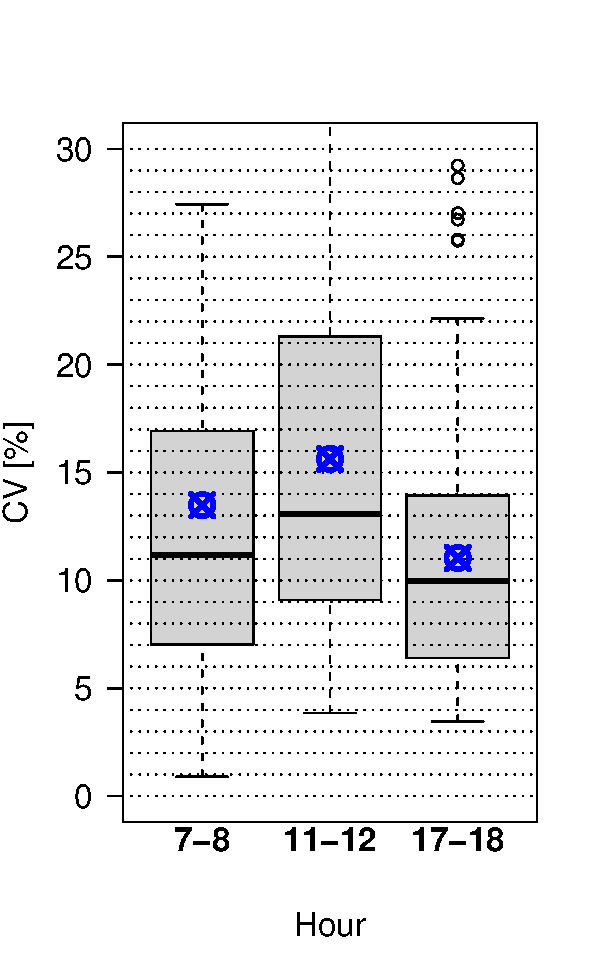
\includegraphics[width=0.3\textwidth]{understanding/figures/var/linkVolumesInter200.pdf}}%
	%{\label{fig:linkVolumesInter200}}%
  %{}%
%}%
%{} 
%
%\vfill\eject
% ##################################################################################################################
% Local Variables:
% mode: latex
% mode: reftex
% mode: visual-line
% TeX-master: "main"
% comment-padding: 1
% fill-column: 9999
% End: 
